\documentclass[twoside,12pt,fleqn]{report}% dvoustranný tisk
%\documentclass[12pt]{report}% jednostranný tisk
% všechny soubory jsou v utf-8. 
	\usepackage{ucs}% pro kódování UTF-8
	\usepackage[utf8x]{inputenc}% kódování vstupních souborů je utf-8
	\PrerenderUnicode{ěščřžýáíéĚŠČŘŽÝÁÍÉďťňĎŤŇůúÚóÓ} %predkresleni diakritiky, mozno pridat/ubrat znaky podle potreby
% pokud si je překódujete např do windows 1250 použijte místo předchozích tří řádků následující:
%\usepackage[cp1250]{inputenc}% kódování vstupních souborů
							                  

\usepackage[czech]{babel}% čeština
%\usepackage[slovak]{babel}% slovenština
\usepackage[IL2]{fontenc}% csr fonty (pokud jsou nainstalovány česká postscriptová mísma)
%\usepackage[T1]{fontenc}% EC fonty - háčky a čárky jsou k písmenkům připojovány - nehezké


\usepackage[]{diplomka}
\usepackage[]{VSKP} % Sablona dle smernice rektora
\input{VSKP} % Uvodni desky atd dle smernice rektora
\splithyphens% při rozdělování slov se spojovníkem opakuj spojovník
\ifx\pdfcompresslevel\undefined
   \usepackage{graphicx}
   \DeclareGraphicsExtensions{.bmp,.eps,.png}
\else
   \usepackage[pdftitle={\typpracetxt},
            pdfauthor={\autortxt},
            pdftex=true,
            %bookmarks=true,
            linkcolor=blue,
            colorlinks=true,
            breaklinks=true,
            a4paper]{hyperref}
   \usepackage[pdftex]{graphicx}
   \DeclareGraphicsExtensions{.png,.pdf}
\fi
\usepackage{amsmath}
\usepackage{mathtools}
\usepackage{alize} %moje styly

%\usepackage{listings}
%\lstset {breaklines=true}
\usepackage{fancyvrb}

\usepackage{rotating}
\usepackage{multirow}


\begin{document}

\titul% vytiskne titul práce
\abstrakty% vytiskne stránku s abstrakty


\prohlaseni{Prohlašuji, že jsem to všechno opsal a vlastními chybami opatřil.}% prohlášení,
\podekovani{Děkuji všem, kteří mi pomohli okopírovat to, co jsem potom opsal.}% poděkování, nepovinné

% vlastní práce
\obsah% vytiskne obsah

%
%  vlastni text
%
\input{Uvod}% nutné
%
% sem vlastni opsany text, možno vložit více souborů (nejlépe pro každou kapitolu zvláštní soubor)
\chapter{Goertzelův algoritmus}
\label{kap:goertzeluvalgoritmus}

\section{Diskrétní Fourierova řada}

Máme řadu $N$ hodnot libovolné posloupnosti. Fourier ukázal, že je možno převést
ji na $N$ hodnot nějaké frekvenční charakteristiky. \emph{Diskrétní Fourierova řada} přiřazuje časové periodické posloupnosti periody $N$,
posloupnost spektra, rovněž periodickou a rovněž periody $N$. Následující vzorec pochází z knihy \emph{Systémy a signály} od prof. Smékala\cite{smekal}.

\begin{myequation}
S_p[k] = \sum_{n=0}^{N-1} s_p[n] \eul^{-\jmag  k\frac{2\pi}{N}n},
\end{myequation}
\noindent kde \emph{k} $k.$ hodnota amplitudy ve spektru, nabývá hodnot $0..N-1, N$ je délka sekvence časové posloupnosti i délka spektra \emph{DFŘ}.
Řada má tedy určitý, omezený počet členů.

\section{Diskrétní Fourierova transformace - DFT}


Na rozdíl od \emph{DFŘ}, není obraz \emph{DFT} periodický. \emph{DFT} přiřazuje
časové posloupnosti délky $N$, posloupnost spektra, také délky $N$. S pomocí
\emph{DFŘ} by se vytvořil asi takto:
\begin{itemize}
\item Zperiodizování průběhu $s$, kde $s[n+lN] = s_p[n]$
\item Výpočet DFŘ.
\item Oříznutí spektra na jednorázovou posloupnost. 
\end{itemize}

\emph{DFT} zapisujeme jako

\begin{myequation}
\label{vztah:DFT}
S[k] = \sum_{n=0}^{N-1} s[n] \eul^{-\jmag  k\frac{2\pi}{N}n}.
\end{myequation}

I tento vzorec pochází z knihy prof. Smékala (\cite{smekal}).

\section{Goertzelův algoritmus}

Často je třeba řešit požadavek na zjištění složky spektra u určitém úzkém pásmu kmitočtů. Šlo by samozřejmě spočítat Fourierovou transformací celé spektrum a~vybrat jen ten kmitočet, který je pro nás zajímavý.
Další možností je spočítání jedné hodnoty z definice Fourierovy transformace, tak jako ve vzorci pro DFT (\ref{vztah:DFT}).
Myšlenkou \emph{Goertzelova algoritmu} je k tomuto účelu použít číslicové filtrace.
Goertzel použil druhou kanonickou strukturu (\ref{vztah:2kanonickastruktura}), realizovanou filtrem IIR (na obrázku \ref{obr:2kanonicka}).

\begin{myequation}
\begin{multlined}
\label{vztah:2kanonickastruktura}
v_1[n+1] = v_2[n] \\
v_2[n+1] = \frac{1}{b_2}(x[n]-b_1v_2[n]-b_0v_1[n]) \\
y[n] = a_2v_2[n+1] + a_1v_2[n] +a_0v_1[n] 
\end{multlined}
\end{myequation}

\begin{figure}
  \begin{center}
    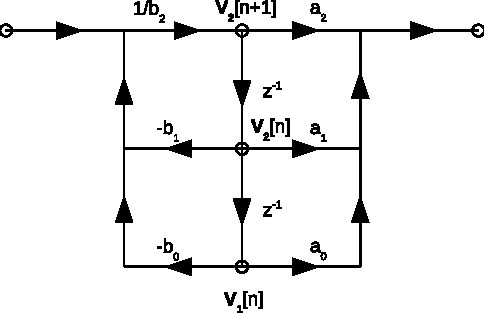
\includegraphics[scale=1]{obr/2kanonickastruktura}
  \end{center}
  \caption{Graf signálových toků druhé kanonické struktury.}
  \label{obr:2kanonicka}
\end{figure}


\section{Odvození Goertzelova algoritmu}

Následující odvození pochází rovněž z knihy prof. Smékala Systémy a signály \cite{smekal}.
\\
 Označme:

\begin{myequation}
\label{vztah:wn}
W_N = \eul^{-\jmag  \frac{2\pi}{N}},
\end{myequation}

pak

\begin{myequation}
\label{vztah:wnrovnost}
(W_N)^{-kN} = (\eul^{-\jmag  \frac{2\pi}{N}})^{-kN} = 1,
\end{myequation}

Protože člen (\ref{vztah:wnrovnost}) je jedna, můžeme s ním vynásobit definiční vztah Fourierovy transformace (\ref{vztah:DFT}), aniž by došlo ke změně.

\begin{myequation}
\begin{multlined}
\label{vztah:geotrzelsk}
S[k] = \sum_{m=0}^{N-1} s[m] W_N^{-kN} = (W_N)^{-kN} \sum_{m=0}^{N-1} s[m] W_N^{-kN} =\\
=\sum_{m=0}^{N-1} s[m] W_N^{-k(N-m)} = \sum_{m=0}^{N-1} s[m] \eul^{-\jmag\frac{2\pi}{N}k(N-m)}
\end{multlined}
\end{myequation}

Konečný tvar vztahu (\ref{vztah:geotrzelsk}) zjevně vypadá jako konvoluce
vstupní posloupnosti $x[n] = s[n]$ s impulsní charakteristikou číslicového filtru typu IIR


\begin{myequation}
\label{vztah:gertzelimpchar}
h[n] =  \eul^{-\jmag  k\frac{2\pi}{N}} = W_N^{-kN} = 1, n = 0,1,2..\infty
\end{myequation}

Impulsní charakteristika má komplexní koeficienty, což je zřejmé i z toho, že
spektrum DFT je také komplexní. Výstupní odezva potom je

\begin{myequation}
\begin{multlined}
\label{vztah:geotrzelyn}
y[n] = x[n]*h[n] = \sum_{m=0}^{\infty} s[m] h[n-m] = \sum_{m=0}^{\infty} s[m] W_N^{-k(n-m)} = \\
\sum_{m=0}^{\infty} s[m] \eul^{-\jmag k\frac{2\pi}{N}(n-m)}
\end{multlined}
\end{myequation}

Tento vzorec (\ref{vztah:geotrzelyn}) je ovšem nekonečná řada. Naštěstí není nutné
počítat do nekonečna, jelikož v hledané spektrální složce je jediný vzorek v čase $N$ roven

\begin{myequation}
\begin{multlined}
\label{vztah:geotrzelopak}
y[N] = \sum_{m=0}^{\infty} s[n] \eul^{-\jmag k\frac{2\pi}{N}(N-m)} =
\sum_{m=0}^{\infty} s[n] \eul^{-\jmag k\frac{2\pi}{N}N} \eul^{-\jmag k\frac{2\pi}{N}m} =
\sum_{m=0}^{N-1} s[n] \eul^{-\jmag k\frac{2\pi}{N}m} =\\
 S[k]
\end{multlined}
\end{myequation}

Přenosová charakteristika filtru typu IIR s impulsní charakteristikou (\ref{vztah:gertzelimpchar}) je prvního řádu

\begin{myequation}
\begin{multlined}
\label{vztah:geotrzelhz}
H(z) = \sum_{n=0}^{\infty} h[n]z^{-n} =  \sum_{n=0}^{\infty} \eul^{-\jmag k\frac{2\pi}{N}n} z^{-n}= \sum_{n=0}^{\infty} ( \eul^{-\jmag k\frac{2\pi}{N}} z^{-1} )^{n} =\\
 \frac{1}{1-\eul^{-\jmag k\frac{2\pi}{N}}z^{-1}} = \frac{z}{z-W_N^{-k}}
\end{multlined}
\end{myequation}

Nevýhodou zcela jistě je skutečnost, že se v přenosové funkci vyskytují komplexní
koeficienty. Následující úprava vztahu (\ref{vztah:geotrzelhz}) tohle řeší. Daň za
možnost práce s jen reálnými čísly je přenosová funkce druhého řádu.

\begin{myequation}
\begin{multlined}
\label{vztah:geotrzelodvoz}
H(z) = \frac{1}{1-W_N^{-k}z^{-1}} = \frac{1}{1-W_N^{-k}z^{-1}} . \frac{1-W_N^{k}z^{-1}}{1-W_N^{k}z^{-1}} =\\
 \frac{1}{1-\eul^{-\jmag k\frac{2\pi}{N}z^{-1}}}
. \frac{1-\eul^{-\jmag  k\frac{2\pi}{N}z^{-1}}}{1-\eul^{-\jmag  k\frac{2\pi}{N}z^{-1}}} =
\frac{1-\eul^{-\jmag  k\frac{2\pi}{N}z^{-1}}}{1 - (\eul^{-\jmag  k\frac{2\pi}{N}+\eul^{-\jmag k\frac{2\pi}{N}})z^{-1} +z^{-2}}} = \\
\frac{1-\eul^{-\jmag  k\frac{2\pi}{N}z^{-1}}}{1-2\cos{k\frac{2\pi}{N}}z^{-1}+z^{-2}} =
\frac{z^{2}-\eul^{-\jmag  k\frac{2\pi}{N}z}}{z^{2}-2\cos{k\frac{2\pi}{N}}z+1} = 
\frac{a_2z^{2}+a_1z+a_0}{b_2z^{2}+b_1z+b_0}
\end{multlined}
\end{myequation}

Výsledek porovnáme se stavovými rovnicemi (\ref{vztah:2kanonickastruktura}) A zjistíme tak následující koeficienty.

\begin{myequation}
\begin{aligned}
\label{vztah:geotrzelkoef}
b_2 &= 1,&&\\
b_1 &= -2\cos{k\frac{2\pi}{N}},&&\\
b_0 &= 1,&&\\
a_2 &= 1,&&\\
a_1 &= -\eul^{-\jmag  k\frac{2\pi}{N}},&&\\
a_0 &= 0
\end{aligned}
\end{myequation}


Jejich dosazením  do (\ref{vztah:2kanonickastruktura}) dostaneme...

\begin{myequation}
\begin{aligned}
\label{vztah:geortzelstavrovnice}
v_1[n+1] &= v_2[n], &&\\
v_2[n+1] &= x[n]+2\cos{k\frac{2\pi}{N}}v_2[n]-v_1[n], &&\\
y[n] &= v_2[n+1] -(\cos{k\frac{2\pi}{N}} -\jmag  \sin{k\frac{2\pi}{N}}) v_2[n], &&\\
\end{aligned}
\end{myequation}


\begin{figure}
  \begin{center}
    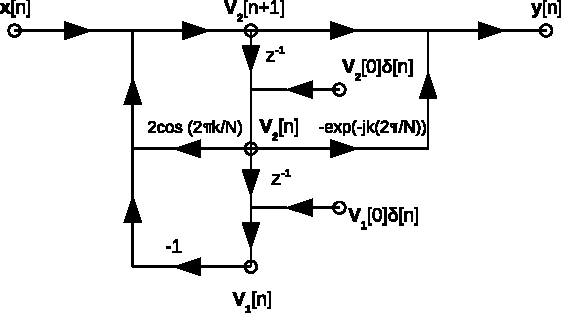
\includegraphics[scale=1]{obr/goertzel}
  \end{center}
  \caption{Graf signálových toků Goertzelova algoritmu ve 2. kanonické struktuře.}
  \label{obr:goertzelova2kanonicka}
\end{figure}

Výhodou této struktury je, že nám stačí ve smyčce počítat jen proměnné
$v_1$ a $v_2$. Výstup $y$ se počítá jen jednou, při posledním průchodu cyklem, kdy $n=N$. Počáteční hodnoty $v_1$ a $v_2$ jsou nulové. Komplexní operace tak bude
provedena pouze jednou a to až na závěr.
\chapter{Možnosti paralelizace}
\label{kap:moznostireseni}

\section{Rozdělení na $N$-částí a jejich průměrování}

Jako první nápad je, aby každé jádro procesoru zpracovávalo poměrnou část výpočtu.
Dostali bychom $N$ výsledků (kde je $N$-počet jader procesoru) a z těch by se udělal
průměr. Jenže z $N$-krát méně vzorků pro výpočet by znamenalo také $N$-krát širší pásmo, které zkoumám. Filtr IIR je totiž pásmová propust. Abych měřil co nejpřesněji, musí být co nejužší. To znamená $N$-krát menší přesnost. Průměrování to zcela jistě nespraví. Navíc se tím neušetří žádný výpočet. Proto dále nebudu v této úvaze pokračovat.

\section{Variace stavové proměnné}

V našem případě by bylo výhodnější, kdybych mohl počítat s neznámými stavovými proměnnými.
Ty totiž počítá jiné jádro. Řekněme, že začínám $n$-tým vzorkem, počítám pro 4 hodnoty $x[n]$, ve stavových proměnných  $v_1$ a $v_2$ mám neznámé hodnoty  $R$ a $S$.

\begin{myequation}
\begin{aligned}
\label{vztah:mojevariacestav}
v_1[n] &= R, &&\\
v_2[n] &= S, &&\\
2\cos{k\frac{2\pi}{N}} &= C &&\\
v_1[n+1] &= v_2[n] =S, &&\\
v_2[n+1] &= x[n]+2\cos{k\frac{2\pi}{N}}v_2[n]-v_1[n] = x[n]+CS-R, &&\\
v_1[n+2] &= v_2[n+1] = x[n]+CS-R, &&\\
v_2[n+2] &= x[n+1]+2\cos{k\frac{2\pi}{N}}v_2[n+1]-v_1[n+1] = &&\\  & x[n+1]+C(x[n]+CS-R)-S =&&\\ &
x[n+1]+Cx[n]+(C^2-1)S-CR, &&\\
v_1[n+3] &= v_2[n+2] =  &&\\& 
x[n+1]+Cx[n]+(C^2-1)S-CR,
\end{aligned}
\end{myequation}

\begin{myequation*}
\begin{aligned} 
v_2[n+3] &= x[n+2]+2\cos{k\frac{2\pi}{N}}v_2[n+2]-v_1[n+2] =  &&\\  & 
x[n+2]+C(x[n+1]+Cx[n]+(C^2-1)S-CR)&&\\&- x[n]-CS+R=&&\\& 
x[n+2]+Cx[n+1]+(C^2-1)x[n]+CS(C^2-2)-&&\\&(C^2-1)R &&\\
v_1[n+4] &= v_2[n+3] =  &&\\& 
x[n+2]+Cx[n+1]+(C^2-1)x[n]+CS(C^2-2)-&&\\&(C^2-1)R &&\\
v_2[n+4] &= x[n+3]+2\cos{k\frac{2\pi}{N}}v_2[n+3]-v_1[n+3] = &&\\  & 
x[n+3]+C(x[n+2]+Cx[n+1]+(C^2-1)x[n]+&&\\&
CS(C^2-2)-(C^2-1)R)-x[n+1]-Cx[n]-&&\\&
(C^2-1)S+CR = &&\\&
x[n+3]+Cx[n+2]+(C^2-1)x[n+1]+C(C^2-2)x[n]+  &&\\&
(C^4-2C^2-C^2+1)S-(C^3-2C)R
\end{aligned}
\end{myequation*}

Zcela zjevně se dají naše dvě neznámé stavové proměnné nahradit třemi novými,
zato známými. Každá rovnice se totiž dá nahradit výrazy:

\begin{myequation}
\begin{aligned}
\label{vztah:mojevariacestavdosazeni}
v_1[n+1] &= v_2[n] = w_0[n] + w_1[n]S-w_2[n]R, &&\\
v_2[n+1] &= x[n] +Cv_2[n] - v_1[n] =&&\\& w_0[n+1] + w_1[n+1]S +w_2[n+1]R, &&\\
\end{aligned}
\end{myequation}
  
Vyskytuje se tu řada: $1,C,C^2-1,C^3-2C,C^4-2C^2-C^2+1,C^5-3C^3+C-C^3+2C$

Při bližším prozkoumání této řady vidím, že má určitou zákonitost.
Založím si tedy novou stavovou proměnnou, nazvu ji $w_3$. Začnu...
\begin{myequation}
\begin{aligned}
\label{vztah:mojevariacestavw3}
w_3[-1] &= 0 &&\\
w_3[0] &= 1 &&\\
w_3[1] &= C &&\\
... &&\\
w_3[n+1] &=  Cw_3[n]-w_3[n-1]&&\\
... &&\\
w_3[2] &= Cw_3[1]-w_3[0] = C^2-1&&\\
w_3[3] &= Cw_3[2]-w_3[1] = C(C^2-1)-C = C^3-2C&&\\
w_3[4] &= Cw_3[3]-w_3[2] = C(C^3-2C)-(C^2-1) =&&\\& C^4 - 3C^2 + 1&&\\
w_3[5] &= Cw_3[4]-w_3[3] = C(C^4 - 3C^2 + 1)-(C^3-2C) =&&\\&
C^5-3C^3+C-C^3+2C=C^5-4C^3+3C
\end{aligned}
\end{myequation}

Pokud zkombinuji rovnice (\ref{vztah:mojevariacestav}) a (\ref{vztah:mojevariacestavdosazeni}), můžu si vyjádřit nové stavové proměnné
$w_1$, $w_2$ a $w_3$. Začnu s $w_0$:

\begin{myequation}
\begin{aligned}
\label{vztah:mojevariacestavw0_1}
w_0[n] &= 0 &&\\
w_0[n+1] &= x[n] &&\\
w_0[n+2] &= x[n+1]+Cx[n] &&\\
w_0[n+3] &= x[n+2]+Cx[n+1]+(C^2-1)x[n]&&\\
w_0[n+4] &= x[n+3]+Cx[n+2]+(C^2-1)x[n+1]+C(C^2-2)x[n]
\end{aligned}
\end{myequation}

Což mohu vyjádřit stavovou proměnnou $w_3$

\begin{myequation}
\begin{aligned}
\label{vztah:mojevariacestavw0_2}
w_0[n+1] &= w_3[0]x[n]&&\\
w_0[n+2] &= w_3[0]x[n+1] + w_3[1]x[n]&&\\
w_0[n+3] &= w_3[0]x[n+2] + w_3[1]x[n+1] + w_3[2]x[n]&&\\
w_0[n+4] &= w_3[0]x[n+3] + w_3[1]x[n+2] + w_3[2]x[n+1] + w_3[3]x[n]&&\\
\end{aligned}
\end{myequation}

Zkusím to opět rozložit podle vzorce (\ref{vztah:mojevariacestavw3}),což vede na původní tvar. Rovnice lze ale přeskládat tak, abych se dostal k rekurentní formuli.
\\
\begin{myequation}
\begin{aligned}
w_0[n+1] &= w_3[0]x[n]=x[n]&&\\
w_0[n+2] &= w_3[0]x[n+1] + (Cw_3[0]-w_3[-1])x[n] = &&\\&
Cw_3[0]x[n] + w_3[0]x[n+1] - w_3[-1]x[n] =&&\\&
Cw_0[n+1]+x[n+1]&&\\
w_0[n+3] &= w_3[0]x[n+2] + w_3[1]x[n+1] + (Cw_3[1]-w_3[0])x[n]=&&\\&
w_3[0]x[n+2] +(Cw_3[0]-w_3[-1])x[n+1] + (Cw_3[0]-&&\\&
w_3[-1])Cx[n]-w_3[0]x[n]=&&\\&
x[n+2]+C(x[n+1]+Cx[n])-x[n] =&&\\&
x[n+2] + Cw_0[n+2]-w_0[n+1]&&\\
w_0[n+4] &= w_3[0]x[n+3] + w_3[1]x[n+2] + w_3[2]x[n+1] + &&\\&
w_3[3]x[n] = x[n+3]+(Cw_3[0]-w_3[-1])x[n+2]+(Cw_3[1]&&\\&
-w_3[0])x[n+1]+(Cw_3[2]-w_3[1])x[n]=&&\\&
x[n+3]+Cx[n+2]+(C^2-1)x[n+1]+(C^3-2C)x[n]=&&\\&
x[n+3]+C(x[n+2]+Cx[n+1]+C^2x[n]-x[n])-&&\\&
Cx[n]-x[n+1] = x[n+4]+Cw_0[n+3]-w_0[n+2]
\end{aligned}
\end{myequation}

Pokračuji s $w_1$:

\begin{myequation}
\begin{aligned}
\label{vztah:mojevariacestavw1_1}
w_1[n] &= 1 = w_3[0]&&\\
w_1[n+1] &= C = w_3[1]&&\\
w_1[n+2] &= C^2-1 = w_3[2]&&\\
w_1[n+3] &= C^3-2C = w_3[3]&&\\
w_1[n+4] &= C^4 - 3C^2 + 1 = w_3[4]
\end{aligned}
\end{myequation}

což je již odvozené $w_3$. Proto tedy mohu napsat

\begin{myequation}
\begin{aligned}
\label{vztah:mojevariacestavw1_2}
w_1[n+1] &=  w_3[1] = Cw_1[0]-w_1[-1]
\end{aligned}
\end{myequation}


A nakonec $w_2$:

\begin{myequation}
\begin{aligned}
\label{vztah:mojevariacestavw2_1}
w_2[n] &= 0 &&\\
w_2[n+1] &= 1&&\\
w_2[n+2] &= C&&\\
w_2[n+3] &= C^2-1&&\\
w_2[n+4] &= C^3-2C
\end{aligned}
\end{myequation}

$w_2$ je posunuté $w_3$

\begin{myequation}
\begin{aligned}
\label{vztah:mojevariacestavw2_2}
w_2[n+1] &=  w_3[n] = w_1[n]
\end{aligned}
\end{myequation}

Ještě je tu malý problém. Rekurentní vzorce pro $w_0$ a $w_1$ se odkazují nejen na poslední člen historie, ale i předposlední. Proto formálně zavedu nové stavové proměnné. Z pohledu procesoru je totiž stejně jedno, zda nějaké paměťové místo nazývám
jako $w_4[n]$ nebo $w_0[n-1]$.

\begin{myequation}
\begin{aligned}
\label{vztah:mojevariacestavodvozene}
w_4[n+1] &= w_0[n]&&\\
w_0[n+1] &= x[n+1]+Cw_0[n]-w_0[n-1] =&&\\& x[n+1] + Cw_0[n] - w_4[n]&&\\
w_2[n+1] &= w_1[n]&&\\
w_1[n+1] &= Cw_1[n]-w_2[n]
\end{aligned}
\end{myequation}

Vztahy pro $w_0$ a $w_4$, které jsem odvodil jsou vlastně vztahy Goertzelova algoritmu
(\ref{vztah:geortzelstavrovnice}). Přibyly jen rovnice pro $w_1$ a $w_2$.
Zajímavé je že $w_1$ a $w_2$ jsou jen konstanty a vůbec nezávisejí na vstupním
signálu. To by ovšem znamenalo zjednodušení spojování těch mezivýsledků, co víc,
$w_1$ a $w_2$ by se vůbec nemusely počítat  v tomto algoritmu, protože jsou již předem známé.


Nyní zkusím malou kontrolu. Zkusím, zda výše uvedené vzorce předpovídají další
hodnotu posloupnosti $v_2$, respektive, zda koeficienty u neznámých $R$ a $S$
jsou z řady $w_3$.

\begin{myequation}
\begin{aligned}
\label{vztah:mojevariacestav3}
v_1[n+5] &= v_2[n+4] =  &&\\& 
x[n+3]+Cx[n+2]+(c^2-1)x[n+1]+C(C^2-2)x[n]+  &&\\&
(C^4-2C^2-C^2+1)S-(C^3-2C)R &&\\
v_2[n+5] &= x[n+4]+2\cos{k\frac{2\pi}{N}}v_2[n+4]-v_1[n+4] = &&\\  & 
x[n+4]+C(x[n+3]+Cx[n+2]+(c^2-1)x[n+1]+&&\\&
C(C^2-2)x[n]+ (C^4-2C^2-C^2+1)S-(C^3-2C)R) - &&\\& 
(x[n+2]+Cx[n+1]+(C^2-1)x[n]+CS(C^2-2)-&&\\&
(C^2-1)R)=&&\\&
[n+4]+Cx[n+3]+(C^2-1)x[n+2]+(c^3-2C)x[n+1]+&&\\&
(C^4-2C^2-C^2+1)x[n]+(C^5-3C^3+C-C^3+2C)S-&&\\&
(C^4-2C^2-C^2+1)R
\end{aligned}
\end{myequation}

A na závěr vyzkouším, zda jsem předpověděl dobře novou stavovou
proměnnou $w_0$.

\begin{myequation}
\begin{aligned}
w_0[n+5] &= w_3[0]x[n+4] + w_3[1]x[n+3] + w_3[2]x[n+2] +&&\\&
w_3[3]x[n+1] + w_3[4]x[n]= &&\\&
x[n+4]+Cx[n+3]+(C^2-1)x[n+2]+&&\\&
(C^3-2C)x[n+1]+(C^4-3C^2+1)x[n]=&&\\&
x[n+4]+C(x[n+3]+Cx[n+2]+C^2x[n+1]-x[n+1]+&&\\&
C^3x[n]-2Cx[n])-(x[n+2]+Cx[n+1]+C^2x[n]-&&\\&
x[n])=x[n+4]+Cw_1[n+4]-w_1[n+3]
\end{aligned}
\end{myequation}

Zkusím tedy malou rekapitulaci výše uvedeného.

Mám signál o $N$ diskrétních hodnotách a chci jej počítat na $P$ procesorových jádrech. Pro jednoduchost budu předpokládat že $N$ je násobek $P$. Vlastně je
úplně jedno, zda bloky, na které $N$-prvkový signál záhy rozdělím, jsou stejně dlouhé.
Každopádně by měly být co možná nejvíce stejně dlouhé, protože celek bude pracovat efektivněji. Jako prerekvizity si spočítám $C= 2 \cos{2 \pi / N}$
a spočítám si $w_1$ a $w_2$, které stačí spočítat jednou v případě, že všech $P$ bloků je stejně dlouhých.
Na každém bloku signálu spočítám hodnoty podle vztahu
(\ref{vztah:mojevariacestavodvozene}) $w_0$ a $w_4$, tedy klasickým způsobem
Goertzelovým algoritmem, bez výpočtu výstupní proměnné $y$. Provedu tedy právě $N$ jednoduchých výpočtů.
Nyní musím mezivýsledky nějak spojit. U každého mezivýsledku znám $w_0$, 
$w_1$ i $w_2$. Mohu tedy napsat v souladu se vztahem (\ref{vztah:mojevariacestavdosazeni}).

\begin{myequation}
\begin{aligned}
R[0] &= 0 &&\\
S[0] &= 0 &&\\
\end{aligned}
\end{myequation}
\begin{myequation}
\begin{aligned}
R[1] &= w_0[0] &&\\
S[1] &= w_4[0] &&\\
\end{aligned}
\end{myequation}
\begin{myequation}
\begin{aligned}
R[2] &= w_0[1] + w_1[1]R[1] - w_2[1]S[1] &&\\
S[2] &= w_4[1] + w_1[1]R[1] - w_2[1]S[1] &&\\
\end{aligned}
\end{myequation}
\begin{myequation}
\begin{aligned}
R[3] &= w_0[2] + w_1[2]R[2] - w_2[2]S[2] &&\\
S[3] &= w_4[2] + w_1[2]R[2] - w_2[2]S[2] &&\\
\end{aligned}
\end{myequation}
\begin{myequation}
\begin{aligned}
R[n+1] &= w_0[n] + w_1[n]R[n] - w_2[n]S[n] &&\\
S[n+1] &= w_4[n] + w_1[n]R[n] - w_2[n]S[n] &&\\
\end{aligned}
\end{myequation}


\section{Maticové operace}
\label{kap:matrixoperations}

Protože budu používat knihovnu openCL, která obvykle využívá výpočetní výkon
grafické karty, je vhodné to nějakým způsobem využít. V grafických výpočtech
se používají matice, druhého, třetího a čtvrtého řádu. Grafický čip je tedy pro
výpočty s těmito maticemi optimalizován. Proto převedu předchozí úvahu do maticové
terminologie. Začnu s přepsáním Goertzelova vztahu (\ref{vztah:geortzelstavrovnice}).
\\
Pro $v[1]$:\\

\begin{myequation}
%\begin{aligned}
v[1] =
\begin{pmatrix}
v_1 [1] \\
v_2 [1]
\end{pmatrix}
= Av[0] + Bx[0]= 
\begin{pmatrix}
0 & 1 \\
-1 & C
\end{pmatrix}
\begin{pmatrix}
v_1 [0] \\
v_2 [0]
\end{pmatrix}
+
\begin{pmatrix}
0 \\
1
\end{pmatrix}
\begin{pmatrix}
x[0] \\
\end{pmatrix}
%\end{aligned}
\end{myequation}
\\
a pro $v[2]$
\\
\begin{myequation}
\begin{multlined}
v[2] =
\begin{pmatrix}
v_1 [2] \\
v_2 [2]
\end{pmatrix}
= A(Av[0] + Bx[0])+Bx[1]= A^2\\ 
\begin{pmatrix}
v_1 [0] \\
v_2 [0]
\end{pmatrix}
+A
\begin{pmatrix}
0 \\
1
\end{pmatrix}
\begin{pmatrix}
x[0] \\
\end{pmatrix}
+
\begin{pmatrix}
0 \\
1
\end{pmatrix}
\begin{pmatrix}
x[1] \\
\end{pmatrix}
\end{multlined}
\end{myequation}
\\
\\
 a nakonec zobecním. Vztah (\ref{vztah:maticovygoertzel}) je Goertzelův algoritmus
 v maticovém zápisu.
 \\

\begin{myequation}
\label{vztah:maticovygoertzel}
\begin{multlined}
v[n+1] =
\begin{pmatrix}
v_1 [n+1] \\
v_2 [n+1]
\end{pmatrix}
= Av[n] + Bx[n]= \\
\begin{pmatrix}
0 & 1 \\
-1 & C
\end{pmatrix}
\begin{pmatrix}
v_1 [n] \\
v_2 [n]
\end{pmatrix}
+
\begin{pmatrix}
0 \\
1
\end{pmatrix}
\begin{pmatrix}
x[n] \\
\end{pmatrix}
\end{multlined}
\end{myequation}
\\
Ten můžu volně přepsat:
\\
\begin{myequation}
\begin{multlined}
v[n+k] = \\
A( A( \dots A( A( A(v[n])+Bx[n] )+Bx[n+1] )+Bx[n+2] )\dots )+\\
Bx[n+k-1]) )+Bx[n+k] 
\end{multlined}
\end{myequation}
\\
Ještě to upravím tak, aby vstup $x$ byl jeden dlouhý sloupcový vektor.
\\
\begin{myequation}
\begin{multlined}
\label{vztah:maticovygoertzelfinal}
v[n+k] = 
\begin{pmatrix}
v_1 [n+k] \\
v_2 [n+k]
\end{pmatrix}
= A^k v[n] + \\
\begin{pmatrix}
A^{k-1}
\begin{pmatrix}
0 \\
1
\end{pmatrix}
& A^{k-2}
\begin{pmatrix}
0 \\
1
\end{pmatrix}
& A^{k-3}
\begin{pmatrix}
0 \\
1
\end{pmatrix}
\dots
\begin{pmatrix}
0 \\
1
\end{pmatrix}
\end{pmatrix}
\begin{pmatrix}
x[n] \\
x[n+1]\\
x[n+2]\\
\vdots \\
x[n+k]
\end{pmatrix}
=\\
A^kv[n]+Dx[n,n+k]^T
\end{multlined}
\end{myequation}

Tento vzorec, když si představím $k=3$, dává jasný návod, jak využít matice čtvrtého řádu. Oproti realizaci elementárními operacemi klesne počet maticových operací na čtvrtinu, protože počítám hned se čtyřmi hodnotami. Rovněž  popisuje spojovaní mezivýsledků z jednotlivých jader. Strana $Dx[n,n+k]^T$ je \emph{Goertzelův} vztah, a je k němu připočten předchozí mezivýsledek vynásobený maticí $A^{k-1}$, tedy konstantou známou před výpočtem. Něco takového jsem již odvodil pro případ počítání po jedné hodnotě $x$ (\ref{vztah:mojevariacestavodvozene}). Samotná matice $D$ je ale také konstanta, která se dá spočítat předem a při konstrukci programu toho využiji.

\section{Počítání hodnot na více kmitočtech současně}
\label{kap:multifrequency}

Předchozí výsledky se dají ještě trochu vylepšit. Prvně nepotřebuji počítat celý horní řádek matice $A^k$. Dostanu z něj předchozí hodnotu a tu vlastně již znám. 
Z toho druhého řádku mám (podle \ref{vztah:multikmitgoertzel}) počítám pro druhý řádek matice $A$ $v_2[n+1] = a_{21}v_1 + a_{22}v_2$. To je nyní první řádek matic ve vztahu \ref{vztah:multikmitgoertzel} s tím, že první index přes čárkou označuje index počítaného kmitočtu. Z maticových operací se stanou vektorové.

Protože ale mám možnost počítat matice čtvrtého řádu, proč nevzít rovnou čtyři
frekvence současně? Začnu s pravou stranou. Protože jsem v minulé větě uvedl, že stačí použít druhý řádek matice $D$, tak teď jej 3-krát zkopíruji do ostatních řádků.
Stejný ale úplně nebude, jelikož konstanta C v sobě zahrnuje kmitočet, takže hodnoty v řádcích budou jiné. Na levé straně u matice $A^k$ provedu to stejné. Vektor $v[n]$
rozšířím také 4-krát, ale do šířky. Výsledkem je matice, říkejme jí $E$, ze které je důležitý jen vektor na diagonále (kde jsou prováděny stejné operace), ostatní hodnoty jsou nenulové ale nejdou pro nás již potřebné.
\\
\begin{myequation}
\label{vztah:multikmitgoertzel}
\begin{multlined}
v[n+3] = 
\begin{pmatrix}
v_{1,2} [n+3] \\
v_{2,2} [n+3] \\
v_{3,2} [n+3] \\
v_{4,2} [n+3]
\end{pmatrix}
= \\
\rm diag \left(
\begin{pmatrix}
a_{1,21}^k & a_{1,22}^k \\
a_{2,21}^k & a_{2,22}^k \\
a_{3,21}^k & a_{3,22}^k \\
a_{4,21}^k & a_{4,22}^k \\
\end{pmatrix}
\cdot
\begin{pmatrix}
v_{1,1} & v_{2,1} & v_{3,1} & v_{4,1}\\
v_{1,2} & v_{2,2} & v_{3,2} & v_{4,2}
\end{pmatrix}
\right) +\\
\begin{pmatrix}
C_1^3 - 2C_1 & C_1^2-1 & C_1 & 1 \\
C_2^3 - 2C_2 & C_2^2-1 & C_2 & 1 \\
C_3^3 - 2C_3 & C_3^2-1 & C_3 & 1 \\
C_4^3 - 2C_4 & C_4^2-1 & C_4 & 1 \\
\end{pmatrix}
\cdot
\begin{pmatrix}
x[n] \\
x[n+1]\\
x[n+2]\\
x[n+3]
\end{pmatrix}
\end{multlined}
\end{myequation}
\\
$\rm diag(A^kv[n])$ jde ještě vyjádřit jako součet dvou vektorů.
\\
\begin{myequation}
\begin{multlined}
v[n+3] = 
\begin{pmatrix}
v_{1,2} [n+3] \\
v_{2,2} [n+3] \\
v_{3,2} [n+3] \\
v_{4,2} [n+3]
\end{pmatrix}
=
\begin{pmatrix}
a_{1,21}^k \\
a_{2,21}^k \\
a_{3,21}^k \\
a_{4,21}^k \\
\end{pmatrix}
\cdot
\begin{pmatrix}
v_{1,1} & v_{2,1} & v_{3,1} & v_{4,1}
\end{pmatrix}
+\\
\begin{pmatrix}
a_{1,22}^k \\
a_{2,22}^k \\
a_{3,22}^k \\
a_{4,22}^k \\
\end{pmatrix}
\cdot
\begin{pmatrix}
v_{1,2} & v_{2,2} & v_{3,2} & v_{4,2}
\end{pmatrix}
+\\
\begin{pmatrix}
C_1^3 - 2C_1 & C_1^2-1 & C_1 & 1 \\
C_2^3 - 2C_2 & C_2^2-1 & C_2 & 1 \\
C_3^3 - 2C_3 & C_3^2-1 & C_3 & 1 \\
C_4^3 - 2C_4 & C_4^2-1 & C_4 & 1 \\
\end{pmatrix}
\cdot
\begin{pmatrix}
x[n] \\
x[n+1]\\
x[n+2]\\
x[n+3]
\end{pmatrix}
\end{multlined}
\end{myequation}

Kde první index je vždy číslo kmitočtu, druhý je index matice původní, neupravené ve vzorci \ref{vztah:maticovygoertzelfinal}.
\chapter{Knihovna openCV}
\label{kap:opencv}

\section{Úvod do openCV}
OpenCV (Open Source Computer Vision Library) dostupná na http://opencv.org \cite{opencv} je open-source BSD-licencovaná knihovna, která zahrnuje několik set algoritmů z počítačového vidění. 
\\
OpenCV má modulární strukturu, jsou v ní zejména moduly uvedené níže:

\begin{itemize}
\item \emph{core} - Základní datové struktury a funkce, zejména pak třída \classname{Mat}.
\item \emph{imgproc} - Filtrace, geometrické transformace a barevné konverze.
\item \emph{video} - Výpočet rozdílu snímků a detekce pohybu.
\item \emph{calib3d} - Základní víceobrazové geometrické transformace.
\item \emph{features2D} - Detektory charakteristických rysů a jejich srovnávače .
\item \emph{objdetect} - Detekce objektů a jejich zařazení do tříd (lidé, oči, obličeje, auta...).
\item \emph{highgui} - Jednoduché uživatelské rozhraní a a interface pro zachytávání obrazu, obrazové a video kodeky. 
\item \emph{gpu} - GPU akcelerované algoritmy ostatních zde uvedených modulů.
\item \emph{ a další...}
\end{itemize}


\section{Základní API}


Knihovna open cv je umístěna ve jmenném prostoru \classname{cv}.
Je to velmi důležité, protože řada jmen funkcí může být stejná jako u jiných knihoven.
Asi nejdůležitější třídou je třída \classname{Mat} reprezentující obecnou matici, se kterou se pracuje téměř stejně jako v programech \srcfilename{matlab}, \srcfilename{octave}. Je tu ale jeden zásadní rozdíl. Třída nemá svoje data, přesněji, několik instancí třídy \classname{Mat} 
může sdílet stejná data. Je to výhodné, protože ve většině případů se tak zamezí kopírování mnoha bytů. Pokud tedy potřebujeme skutečně Matici zkopírovat, použijeme její členskou metodu \functionname{clone}.
Je třeba upřesnit, že \classname{Mat} může být i jen určitá oblast jiné \classname{Mat} a přesto sdílejí společná data. \classname{Mat} definuje možnost mít jako data většinu základních typů, samozřejmě jako \classname{unsigned char}, \classname{signed char}, \classname{usigned short}, \classname{float}, \classname{double}, a  další. Umí samozřejmě několik kanálů. Uvedu krátký příklad:


\begin{Verbatim}
// vytvoří  8MB velkou matici
Mat A(1000, 1000, CV_64F);

// vytvoří jinou hlavičku pro stejná data
Mat B = A;
\end{Verbatim}


\begin{Verbatim}
// vytvoří jinou hlavičku, jako třetí řádek matice A.
// žádná data se nekopírují
Mat C = B.row(3);
\end{Verbatim}


\begin{Verbatim}
// teď vytvoří samostatnou kopii matice B
Mat D = B.clone();
\end{Verbatim}

\begin{Verbatim}
// zkopíruje 5tý řádek matice B do matice C,
// matice C nyní bude mít stejná data jako matice A.
B.row(5).copyTo(C);
\end{Verbatim}


\begin{Verbatim}
// teď A a D sdílí stejná data. Matice B a C ale stále ukazují na data
// staré modifikované matice A
A = D;
\end{Verbatim}


\begin{Verbatim}
// nyní smažeme referenci na data u matice B. Matice C
// ale stále ukazuje na data staré modifikované matice
// A. A to přesto, že ukazuje jen na jeden osamocený řádek těchto dat.
B.release();;
\end{Verbatim}


\begin{Verbatim}
// nakonec, vytvořením úplné kopie matice C zaručíme,
// že původní data budou dealokované, protože
// žádné matice na ně již nebude držet odkaz.
C = C.clone();
\end{Verbatim}
 

Matice se dá snadno vypsat, stačí jí poslat do výstupního streamu.

\begin{Verbatim}
cout<<R;

//nebo

cout << "R (python)  = " << endl << format(R,"python") << endl << endl;
\end{Verbatim}

%\section{První projekt}
%
%Tento projekt, takový \uv{Hello openCV world} jsem si vypůjčil ze
%stránek \url{openCV.org}. Demonstruje, že začít projekt s openCV je skutečně jednoduché. Jsou  v něm použity pouhé 4 funkce: načtení obrázku, jehož jméno
%je dáno jako parametr z~příkazové řádky(\functionname{imread}), potom vytvoření okna (\functionname{namedWindow}) následně zobrazení obrázku v okně (\functionname{imshow}) a nakonec jen čekání na stisk klávesy (\functionname{waitKey}).
%\\
%\srcfilename{Main.cpp}:
%
%\begin{Verbatim}
%#include <stdio.h>
%#include <opencv2/opencv.hpp>
%
%using namespace cv;
%
%int main(int argc, char** argv )
%{
%    if ( argc != 2 )
%    {
%        printf("usage: DisplayImage.out <Image_Path>\n");
%        return -1;
%    }
%
%    Mat image;
%    image = imread( argv[1], 1 );
%
%    if ( !image.data )
%    {
%        printf("No image data \n");
%        return -1;
%    }
%    namedWindow("Display Image", WINDOW_AUTOSIZE );
%    imshow("Display Image", image);
%
%    waitKey(0);
%
%    return 0;
%}
%\end{Verbatim}
%
%Pro překlad je třeba vytvořit si následující soubor:	
%\\
%\srcfilename{CMakeLists.txt}
%
%\begin{Verbatim}
%
%cmake_minimum_required(VERSION 2.8)
%project( test02 )
%find_package( OpenCV REQUIRED )
%add_executable( dist/Debug/GNU-Linux/test02 main.cpp )
%target_link_libraries( dist/Debug/GNU-Linux/test02 \${OpenCV_LIBS} )
%\end{Verbatim}
%\label{sec:compilerules}
%\noindent
%kde test02 je jméno projektu a výstupního spustitelného souboru.
%Pak lze přidat výše uvedený zápis  kamkoliv do projektu.
%Spuštění provádímě jako každého jiného programu, s tím rozdílem, že je třeba nejdříve projekt
%přeložit příkazem \srcfilename{cmake}.
%
%\begin{Verbatim}
%cmake .
%make
%dist/Debug/GNU-Linux/test02 lena.jpg
%\end{Verbatim}

%
%\input{Zaver}% nutné
\input{Literatura}% nutné
\chapter{Instalace projektu - spuštění aplikace}
\label{kap:instalaceprogramu}

K aplikaci není přiložen žádný instalační program. Není potřeba. Spouští se jen spustitelným souborem \emph{SoundAnalyzer} v adresáři téhož jména. Zabalený archiv s~programem naleznete na přiloženém CD disku. Stačí jej jen rozbalit.


Nicméně pro správnou funkci je třeba mít správně nainstalované knihovny \emph{OpenCL} a \emph{OpenGL}. Knihovny \emph{OpenGL} a \emph{OpenCL} dodává výrobce grafické karty, tudíž je problematické napsat nějaký návod na její nainstalování, nebo dokonce nějaký instalační skript. Obecně lze říci, že v linuxu je lepší používat proprietární ovladače od výrobců grafických čipů něž ovladače volně šiřitelné. Jejich instalace ale může přinést potíže, mně třeba pokus o instalaci ovladače od NVidie způsobil nefunkčnost operačního systému a musel jsem tento znovu nainstalovat.

\section{GPU AMD}

Na \url{http://support.amd.com/en-us/download/linux} lze stáhnout ovladač \emph{fglrx}. S jeho instalací jsem neměl žádné problémy. Možná bude potřeba nainstalovat i~\emph{OpenCL} z adresy \href{http://developer.amd.com/tools-and-sdks/opencl-zone/amd-accelerated-parallel-processing-app-sdk/}{developer.amd.com} a je rovněž na přiloženém CD nosiči. Instalace je bez problémů.

\section{GPU NVidia}

Ovladač Nvidia je nyní ve standardním repozitáři Ubuntu a Mint a to v poslední verzi \emph{375}. Když instalujete nové Ubuntu nebo Mint, je třeba před instalací spustit správce ovladačů a vybrat \uv{používat NVidia 340}. Když Linux nainstalujete a připojíte k síti a opět spustíte výše jmenovaný program, nabídne vám již aktuální verzi \emph{375}. OpenCl je součátí CUDA a je také ve standardním repozítáři.
Nainstalujete zadáním:

\begin{Verbatim} 
sudo apt-get install libcuda1-375
\end{Verbatim}

\chapter{Instalace projektu - pokračování ve vývoji}
\label{kap:instalace}

\section{Instalace GNU C++}

Přestože knihovny \emph{OpenCV} a \emph{OpenCL} jsou multiplatformní, rozhodl jsem se pro operační systém Linux, distribuce Mint 17. Vyhnul jsem se konstrukcím platformně závislým, takže je možná přenositelnost na jiné operační systémy. Jako překladač jsem zvolil \emph{GCC}, a to ze stejného důvodu jako předchozí, je platformně nezávislý a~je v každé distribuci Linuxu jako jeden ze základních balíčků. Mně stačilo
k instalaci napsat:

\begin{verbatim}
sudo apt-get install build-essential
\end{verbatim}

a potom...

\begin{Verbatim}
sudo apt-get install g++
\end{Verbatim}


Pro Windows existuje disrtibuce GNU cygwin, kterou je možno stáhnout a nainstalovat z webu \url{sourceware.org/cygwin}.


Důležité je nezapomenout zaškrtnout \emph{devel} a \emph{debug} v seznamu balíčků k instalaci.



\section{Verzovací systém Git}

Verzovací systém Git používám nejen v zaměstnání, ale i v domácích
projektech a~má své místo i v této práci. Může být důležité moci se v případě
nutnosti vrátit k~předchozím verzím projektu.

Git je standardní balíček snad všech distribucí. Instaluje je jako obvykle napsáním

\begin{Verbatim} 
sudo apt-get install git
\end{Verbatim}

S klíči se zachází standardním způsobem, měly by být uloženy v
adresáři \functionname{\textasciitilde/.ssh}.

Vytvořil jsem speciální repozitář na svém testovacím serveru.
Přihlašovat se jde výhradně pomocí klíče, který najdete na CD--příloze této práce. Projekt stačí už jen naklonovat příkazem,

\begin{Verbatim} 
git clone virtualbox@46.167.245.175:dp
\end{Verbatim}

přesněji, pomocí klíče na CD

\begin{Verbatim} 
ssh-agent sh -c 'ssh-add <cesta>/virtualbox_rsa;
git clone virtualbox@46.167.245.175:dp'
\end{Verbatim}


\section{Qt Creator}


Qt Creator je nedílnou součástí vývojového kitu knihovny Qt. Nyní je již verze
5.8, já jsem ale použil verzi 5.5.1, která je podporována ve standardních repozitářích linuxu, konkrétně jsem vyzkoušel Mint 18.1 a Ubuntu 16.04.

Instalační baliček je součástí přiloženého CD a je možné ho rovněž stáhnout ze stránek \url{qt.io}.


Celá aplikace je napsaná v prostředí \emph{Qt Creator}. \emph{Qt creator} má problémy s~vizuálním návrhářem, a to takové, že je zcela nepoužitelný a layout dialogů je nutné psát textově v jazyce /emph{qml}. Stále je však možno použít prostředí \emph{QtCreatoru} pro psaní textu a překlad programu.


\section{OpenGL}


Instalaci proprietárního ovladače a knihovny \emph{OpenGL} jsem popsal v kapitole \emph{instalace programu} \ref{kap:instalaceprogramu}.

Tím ale máme v systému knihovny, nikoli už ale  hlavičkové soubory pro jejich použití. Já jsem napsal pro začátek vývoje v OpenGL toto:

\begin{Verbatim} 
sudo apt-get install freeglut3
sudo apt-get install freeglut3-dev
sudo apt-get install binutils-gold
sudo apt-get install mesa-common-dev
sudo apt-get install libglew1.5-dev libglm-dev
\end{Verbatim}

\section{OpenAL}

Instalace vývojových balíčků pro knihovnu OpenAl je velmi jednoduchá, prakticky nikdy se nestalo že by něco nefungovalo. V Ubuntu jsou to standardní balíčky:

\begin{Verbatim} 
sudo apt-get install libopenal-dev
sudo apt-get install libalut-dev
\end{Verbatim}

\section{OpenCL}

Tak jako \emph{OpenGL} i \emph{OpenCL} je poskytována výrobcem grafického čipu. Je tedy nutné 
mít dobře nainstalovanou grafickou kartu s proprietárními ovladači.

Ve standardních repozitářích Ubuntu je následující balíček...

\begin{Verbatim} 
sudo apt-get install ocl-icd-libopencl1,
\end{Verbatim}

ten nainstaluje nějakou \emph{OpenC}L knihovnu. Program potom jde spustit, ale inicializace vrátí chybu, není platforma, takže není možno provádět výpočet ani softwarově.


SDK pro \emph{OpenCL} na grafických čipech \emph{AMD} je možno stáhnout z adresy \href{http://developer.amd.com/tools-and-sdks/opencl-zone/amd-accelerated-parallel-processing-app-sdk/}{developer.amd.com} a je rovněž na přiloženém CD nosiči. Instalace je bez problémů.
Jediné co potom musíte udělat, je nastavení cesty ke hlavičkovému souboru a knihovně v případě, že chcete použít její vývojovou verzi. U mně to bylo například:\\
\emph{/opt/AMDAPPSDK-2.9-1/include}.


SDK pro \emph{OpenCL} na grafických čipech \emph{NVidia} je v Ubuntu ve standardních repozitářích a
je spojena s implementací knihovny \emph{CUDA}. Pro instalaci stačí napsat:

\begin{Verbatim} 
sudo apt-get install libcuda1-375
sudo apt-get install nvidia-cuda-dev
\end{Verbatim}
kde 375 je jméno verze ovladače grafického čipu NVidia.

\input{SeznamZkratek}% nutné
\chapter{Seznam příloh}
Sem napsat přílohy jestli nějaké jsou
% není povinné
\end{document}
